\documentclass{article}
\usepackage{graphicx} % Required for inserting images
\usepackage{float}
\usepackage{array}
\usepackage{a4wide}
\usepackage{cryptocode}

\begin{document}
\section{current sec model to transcribe ADEM + AMAC to a more symmetric style}
\subsection{used primitives}
\begin{itemize}
    \item ADEM: input fixed length tag, fixed length key and variable length message lead to a variable length cythertext. It should be improbable distinguish the cythertexts of two messages. (adversary may choose two cythertexts and has to guess which one of the two is encrypted). The ADEM gives us access to a enc and a dec call.
    
    \item AMAC: input fixed length tag, fixed length key and variable length message lead to a fixed length cythertext. It should be improbable to make a forgery (a pair (key, tag, message, cythertext) that verifies without begin generated by calling O.mac(key, tag, message) first). The AMAC gives us access to a mac and a ver call.
\end{itemize}

\subsection{goal}
Each user is provided with two keys, a message and a tag that is bound to the user and does not repeat between users. The message is encrypted using the tag and two keys to generate a cythertext consisting of two parts. First part is Cdem which is the message encrypted with the nonce and the first key while the second part is Cmac that is the mac computed over Cdem, the tag and the second key. Given only one queries to Oenc per user and multiple queries to Odec which always occurs after the Oenc queries, the message should be protected against active adversaries as long as DEM and MAC are secure.

\subsection{Sec model}
the security is purely based on the games for the AMAC and ADEM that are visible below. All variables are elaborated in the paper
\begin{figure}[H]
    \centering
    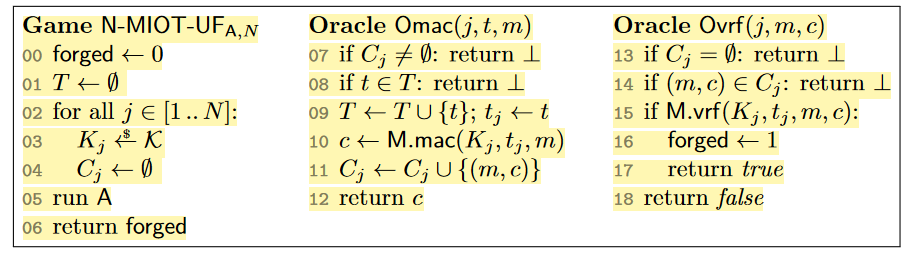
\includegraphics[scale = 0.5]{images/game mac.png}
\end{figure}
\begin{figure}[H]
    \centering
    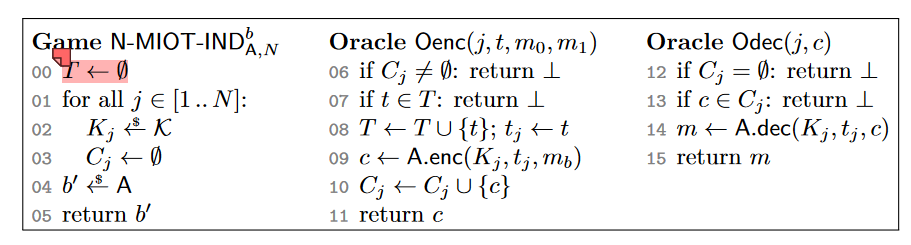
\includegraphics[scale = 0.5]{images/game adem.png}
\end{figure}
with
\begin{figure}[H]
    \centering
    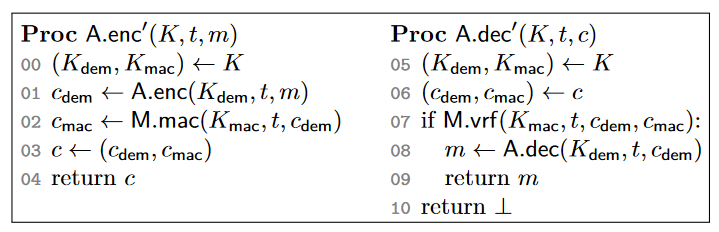
\includegraphics[scale = 0.5]{images/adem amac.png}
\end{figure}


\newpage
\section{needed sec model to transcribe ADEM + AMAC to a more symmetric style}
for now we only look at the nonce based options as the pkc paper does that too.
\subsection{used primitives}
\begin{itemize}
    \item DEM: input fixed length nonce, fixed length key and variable length message lead to a variable length cythertext which should be improbable to distinguish from RO (adversary has to guess if he is talking to RO or DEM). The dem gives us access to a enc and dec call.
    
    \item MAC: input fixed length nonce, fix length key and variable length message lead to a fixed length tag that should be improbable to distinguishable from random oracle (adversary has to guess if he is talking to RO or MAC). The MAC gives us access to a mac call.
\end{itemize}

\subsection{goal}
Each user is provided with two keys, a message and a lock that does not repeat between users. The message is encrypted using the lock and two keys. Given only one queries to Oenc per user and multiple queries to Odec which always occurs after the Oenc queries, the message should be protected against active adversaries as long as DEM and MAC are secure.

\subsection{Sec model}
We define the following sec games for the MAC, the DEM and the DEM+MAC (names will prob be improved later):

\begin{figure}[H]
    \begin{pchstack}[boxed,center,space=0.5cm]
        \pseudocode[lnstart=-1,linenumbering,head={\textbf{Game} MAC$^M_{A,N}$ }]{
        L \leftarrow \emptyset\\
        \pcfor j \in [1..N]:\\
        \t K_j \leftarrow^\$ K\\
        b' \leftarrow A\\
        \pcreturn b'
        }
        \pseudocode[lnstart=4,linenumbering,head={\textbf{Oracle} Omac(j,l,m)}]{
            \pcif T_j \neq \emptyset: \pcreturn \bot\\
            \pcif l \in L: \pcreturn \bot\\
            L \leftarrow L \cup \{l\}\\
            l_j = l\\
            t \leftarrow M.mac(K_j,l_j,m)\\
            \pcreturn t
        }
    \end{pchstack}
\caption{MAC game, M is either the MAC or Random Oracle}
\end{figure}

\begin{figure}[H]
    \begin{pchstack}[boxed,center,space=0.5cm]
        \pseudocode[lnstart=-1,linenumbering,head={\textbf{Game} DEM$^E_{A,N}$ }]{
        L \leftarrow \emptyset\\
        \pcfor j \in [1..N]:\\
        \t K_j \leftarrow^\$ K\\
        b' \leftarrow A\\
        \pcreturn b'
        }
        \pseudocode[lnstart=4,linenumbering,head={\textbf{Oracle} Omac(j,l,m)}]{
            \pcif T_j \neq \emptyset: \pcreturn \bot\\
            \pcif l \in L: \pcreturn \bot\\
            L \leftarrow L \cup \{l\}\\
            l_j = l\\
            c \leftarrow E.enc(K_j,l_j,m)\\
            \pcreturn c
        }
    \end{pchstack}
\caption{DEM game, E is either the DEM or Random Oracle}
\end{figure}

\begin{figure}[H]
    \begin{pchstack}[boxed,center,space=0.5cm]
        \pseudocode[lnstart=-1,linenumbering,head={\textbf{Game} AE$^{AE}_{A,N}$ }]{
        L \leftarrow \emptyset\\
        \pcfor j \in [1..N]:\\
        \t K_j \leftarrow^\$ K\\
        \t C_j \leftarrow \emptyset\\
        b' \leftarrow A\\
        \pcreturn b'
        }
        \pseudocode[lnstart=5,linenumbering,head={\textbf{Oracle} Oenc(j,l,m)}]{
            \pcif T_j \neq \emptyset: \pcreturn \bot\\
            \pcif l \in L: \pcreturn \bot\\
            L \leftarrow L \cup \{l\}\\
            l_j = l\\
            c \leftarrow EA.enc(K_j,l_j,m)\\
            C_j \leftarrow C_j \cup c\\
            \pcreturn t
        }
        \pseudocode[lnstart=12,linenumbering,head={\textbf{Oracle} Odec(j,m)}]{
            \pcif c_j \neq \emptyset: \pcreturn \bot\\
            \pcif c \in C_j: \pcreturn \bot\\
            m \leftarrow EA.dec(K_j,L_j,c)\\
            \pcreturn m
        }
    \end{pchstack}
\caption{AE game, where AE is either the AE scheme having access to the MAC and DEM or RO}
\end{figure}
\noindent We should consider what the RO calls should do, there are several cases to consider:
\begin{itemize}
    \item RO replacing M: RO.mac(k,l,m) calls t = M.mac(k,l,m) then outputs $\bot$ if t is $\bot$ or $|t|$ random bits otherwise.
    \item RO replacing E: RO.enc(k,l,m) calls c = E.enc(k,l,m) then outputs $\bot$ if c is $\bot$ or $|c|$ random bits otherwise.
    \item RO replacing AE: RO.enc(k,l,m) calls c = AE.enc(k,l,m) then outputs $\bot$ if c is $\bot$ or $|c|$ random bits otherwise. RO.dec(k,l,c) always returns $\bot$.
\end{itemize}

\noindent The AE schemes should be constructed from the DEM and the MAC. Following General Composition reconsidered, three ways to construct this EA are of interest, namely the ones following from the N1, N2 and N3 scheme. One thing to keep in mind with this that these schemes would originally use associated data. For now we can discard this but it is not proven that the same security results would also follow from this case without associated data. Down here the initial schemes can be found, followed by the AE.enc and AE.dec calls that can we construct following these schemes.
\begin{figure}[H]
    \centering
    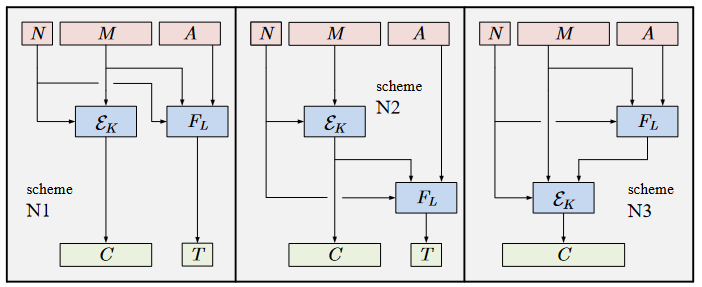
\includegraphics[scale = 0.7]{images/N games.png}
\caption{Original N schemes from Generic Composition reconsidered}
\end{figure}

\begin{figure}[H]
    \begin{pchstack}[boxed,center,space=0.5cm]
        \pseudocode[lnstart=-1,linenumbering,head={EA.enc(k,l,m)}]{
            (k1,k2) \leftarrow k \\
            c' = E.enc(k1,l,m) \\
            t = M.mac(k2,l,m) \\
            c = (c',t)\\
            \pcreturn c
        }
        \pseudocode[lnstart=4,linenumbering,head={EA.dec(k,l,c)}]{
            (k1,k2) \leftarrow k \\
            (c',t) \leftarrow c \\
            m = E.dec(k1,l,c') \\
            t' = M.mac(k2,l,m) \\
            \pcif t = t' : \pcreturn m \\
            \pcelse : \pcreturn \bot
        }
    \end{pchstack}
\caption{Calls based on N1}
\end{figure}

\begin{figure}[H]
    \begin{pchstack}[boxed,center,space=0.5cm]
        \pseudocode[lnstart=-1,linenumbering,head={EA.enc(k,l,m)}]{
            (k1,k2) \leftarrow k\\
            c' = E.enc(k1,l,m)\\
            t = M.mac(k2,l,c')\\
            c = (c',t)\\
            \pcreturn c
        }
        \pseudocode[lnstart=4,linenumbering,head={EA.dec(k,l,c)}]{
            (k1,k2) \leftarrow k\\
            (c',t) \leftarrow c\\
            m = E.dec(k1,l,c')\\
            t' = M.mac(k2,l,c')\\
            \pcif t = t' : \pcreturn m \\
            \pcelse : \pcreturn \bot
        }
    \end{pchstack}
\caption{Calls based on N2}
\end{figure}

\begin{figure}[H]
    \begin{pchstack}[boxed,center,space=0.5cm]
        \pseudocode[lnstart=-1,linenumbering,head={EA.enc(k,l,m)}]{
            (k1,k2) \leftarrow k\\
            t = M.mac(k2,l,m)\\
            m' = m || t\\
            c = E.enc(k1,l,m')\\
            \pcreturn c
        }
        \pseudocode[lnstart=4,linenumbering,head={EA.dec(k,l,c)}]{
            (k1,k2) \leftarrow k\\
            m' = E.dec(k1,l,c)\\
            (m,t) \leftarrow m'\\
            t' = M.mac(k2,l,m)\\
            \pcif t = t' : \pcreturn m \\
            \pcelse : \pcreturn \bot
        }
    \end{pchstack}
\caption{Calls based on N3}
\end{figure}

\newpage
\section{burning questions}
\begin{itemize}
   \item Q1: Is het oke om de games gebazeerd te hebben op RO\\
   Q2:(klopt het dat RO stickt sterker is dan left-right)
   \item Q: in GCrec, waarom zijn er bij de n-schemes geen N4 en N5 schemas? \\ A: die voegen niets toe Q2: klopt dat?
   \item Q: sommige dingen staan twee keer in crypto.bib, is er een voorkeur in welke je cite? \\ A: journal -> procedings -> eprint (make sure that these could differ)
\end{itemize}

\newpage
\section{current todo's}
\begin{itemize}
    \item meer structuur aan brengen in main
    \item verplaatsen naar main
    \item CEASAR GCren people (paper)
    \item add crypto.bib as submodule
    \item change to ind-\$
    \item introduction to modern cryptography katz lindell?
    \item in meer detail opschrijven wat de variables zijn van de sec games en wat de aannamens zijn
    \item mayhabs beginnen met schrijven in main
\end{itemize}

\newpage
\section{main idea}
The PKC paper ends with a ADEM + AMAC construction as "solution". The original paper from ENC -> MAC has been revised, so this should prob be revised as well. In general its nice to write down thing in a more "sym crypto" style as we use symmetric primitives. It would probably also be nice to revise it more in general and see what other ways there are to reach the end-goal expected in the PKC paper.
\end{document}